% !TeX spellcheck = en_GB
\begin{figure}
  \setlength{\unitlength}{\textwidth}

  \begin{picture}(1,0.3)(-0.02,0)
          
    \put(-0.02,0.04){\includegraphics[width=0.5\unitlength]{./chapter-methodology/fnp/vel-amp-convergencexs.eps}}
    \put(0.5,0.04){\includegraphics[width=0.5\unitlength]{./chapter-methodology/fnp/freq-response-convergencexs.eps}}
        
    \put(0.48,0.166){ $ f_{DNS}$ }
    \put(-0.03,0.166){$\displaystyle\dot{y}_{m}$}
    % \put(0.73,0.00){ $\displaystyle\frac{c}{\rho\mathcal{A}U}$}

    \put(0.23,0.03){\emph{p-order}}
    \put(0.75,0.03){\emph{p-order}}
   
    \put(0.071,0.24){\small(a)}
    \put(0.605,0.24){\small(b)}
      
    \end{picture}

    % \caption{Comparison of DNS data. (a) Maximum power obtained using
    %   a 3 point localised quadratic fitting as a function of
    %   \massstiff. (b) \massdamp as a function of \massstiff at maximum
    %   power}

    \caption{Mean velocity amplitude ($\dot{y}_{m}$) (a) and the galloping frequency ($f_{DNs}$) (b) as a function of the interpolation polynomial. Data present $\frac{tU}{D}=0.001$ (\ding{83}) and $\frac{tU}{D}=0.0005$ ($\bullet$). Data acquired  $\reynoldsnumber=200$ $\massdamp=0$ using FSI direct numerical simulations.}

    \label{fig:FSI_convergence}
\end{figure}

 %vspace{10cm}
